\documentclass{article}
\include{graphicx}
\begin{document}

\section{Cosmological Distances}
This section introduces some of the important distances used in various prediction calculations. First of all is the $\textbf{comoving distance}$ between two observers at different redshifts. This is calculated via \cite{distance_measures_cosmology},
\begin{equation}
D_{C}(z)=\frac{c}{H_{0}}\int^{z_{2}}_{z_{1}}\frac{dz'}{E(z')}
\end{equation}
where E(z) is the dimensionless Hubble parameter which is,
\begin{equation}
E(z)=\sqrt{\Omega_{M}(1+z)^{3}+\Omega_{R}(1+z)^{4}+\Omega_{\Lambda}}
\end{equation}
Where $\Omega_{M}$, $\Omega_{R}$ and $\Omega_{\Lambda}$ are the different density parameters for mass, radiation and dark energy respectively.\\
To calculate the comoving distance to an object at a particular redshift the integral above must be done for $z_{1}=0$ up to an arbitrary z. Comoving distance is the distance between two comoving observers i.e. both moving with respect to the Hubble flow (factoring out the expansion of the universe). In the project this has been used to determine a volume of space for a given redshift range. This was done by finding the volume difference between two shells of comoving radius at two different redshifts.\\

The $\textbf{luminosity distance}$ is the distance that a photon travels from a source to an observer. As a photon will undergo a Doppler shift and be redshifted into longer wavelengths (red part of the spectrum). Therefore the luminosity distance is essentially a redshifted transverse comoving distance \cite{distance_measures_cosmology}, which for a flat universe is the comoving distance therefore,
\begin{equation}
D_{L}(z)=(1+z)D_{C}(z)
\end{equation}
In this project the luminosity distance has been used to convert between magnitudes, luminosity and flux.\\

Also, the $\textbf{angular diameter}$ distance is simply the proper distance along a radius $r_{e}$ where this is the radius at the time of emission. Therefore angular diameter distance is,
\begin{equation}
D_{A}=r_{e}a_{e}=\frac{a_{0}r_{e}}{1+z_{e}}
\end{equation}
where $a_{0}r_{e}$ in a flat universe is the same as,
\begin{equation}
D_{A}(z)=\frac{D_{C}}{1+z}
\end{equation}
This is used to convert angular separations in telescope images to actual angular separations and then can determine the size of objects \cite{distance_measures_cosmology}.

\section{Schechter Function}
One important part of our project is to determine the luminosity function at high redshift, which is a plot of the number density of galaxies binned against their respective luminosities. A schechter function is used to fit this luminosity function. A schechter function is a form that has a power law which has a certain cut-off at which it becomes an exponential curve. The schechter function in terms of luminosity i.e. the luminosity function is shown below, \cite{cosmo_number_densities}.
\begin{equation}
\phi(L)=\frac{\phi^{*}}{L^{*}}\frac{L}{L^{*}}^{\alpha}e^{-L/L^{*}}
\label{eq:LumFunc}
\end{equation}
$\phi^{*}$ is the normalization factor in units of $Mpc^{-3}$, $\alpha$ is the gradient of the faint end slope of the luminosity function and $L^{*}$ is the characteristic luminosity at which the function changes from a power law to an exponential cut-off. Therefore there is a majority of lower luminosity galaxies and not many bright ones.\\

There are two basic methods to determine the best fit parameters of the schechter function \cite{luminosity_functions_online}. The first one is to take cluster samples and bin them by apparent magnitude then fit a schechter function trying to minimize the error. The other way is to use the ``maximum likelihood method''. This method takes a flux limited sample and finds the probability that a galaxy actually has a particular luminosity at respective distances and then define a likelihood function which is the joint probability of finding all luminosities at their respective distances. These are then the most likely parameters consistent with the data and a schechter form. However in this project schechter parameters were simply cited from various articles as we are not doing any observations ourselves to get our predictions.\\

The luminosity function can then be integrated to find the number density in $Mpc^{-3}$,
\begin{equation}
\rho_{N}=\int^{\infty}_{L}\phi(L)dL
\end{equation}
Where L is the lower limit luminosity that can be seen in the universe, this is needed as the luminosity function tends to infinity at the faint end.\\
It is easier to plot the luminosity function on the log scale and therefore most of the papers we cite state the absolute magnitude schechter function instead which is obtained by substituting,
\begin{equation}
\frac{L}{L*}=10^{0.4(M^{*}-M)}
\end{equation}
into equation \ref{eq:LumFunc}, which is then multiplied by the derivative and rearranged to get the equation,
\begin{equation}
\phi(M)=\phi^{*}(ln10)\left[10^{0.4(M^{*}-M)}\right]^{\alpha+1}exp\left[-10^{0.4(M^{*}-M)}\right]
\end{equation}
Where $M^{*}$ is the characteristic absolute magnitude where the cut-off happens.\\
However a range of apparent magnitudes is normally observed, rather than absolute magnitudes and so the absolute magnitude equation above is changed to it's apparent magnitude form, using the simple relationship below,
\begin{equation}
m=M+5((log_{10}D_{L})-1)
\end{equation}
Where $D_{L}$ is the luminosity distance. Note that the derivative of this substitution is 1 and so does not need to be accounted for.\\

Or the luminosity density of galaxies in $erg s^{-1}Mpc^{-3}Hz^{-1}$ can also be calculated using,
\begin{equation}
\rho_{L}=\int^{\infty}_{L}L\phi(L)dL
\end{equation}
This will become useful for calculating star formation rates in later sections.\\


\section{Lower Redshift limit on Reionization}
In the project the way that the lower redshift limit has been calculated is to first calculate the rate of photons capable of ionizing a hydrogen atom via the equation, \cite{2010Natur.468...49R}
\begin{equation}
\frac{dn_{ion}}{dt}=f_{esc}\zeta\rho_{SFR}  
\end{equation}
Where $f_{esc}$ is the fraction of ionizing photons that escape a galaxy, $\zeta$ is the number of hydrogen-ionizing photons produced per second per unit star formation rate and $\rho_{SFR}$ is the star formation rate per unit volume.\\

Therefore by integrating this equation up to the age of the universe at a specific redshift a total number of photons capable of ionizing the universe can be outputted. The number of ionizing photons are then equated to the total number of hydrogen atoms in the IGM of the universe to get a lower redshift limit of Reionization.\\
First of all the program gets the critical density of the universe by,

\begin{equation}
\rho_{crit}(z)=\frac{3H(z)^{2}}{8\pi G}
\end{equation}

Then by multiplying this by the baryonic density parameter, $\Omega_{b}=0.045\pm0.004$, the baryonic density is achieved. By then multiplying by the fraction of hydrogen, calculated from big bang nucleosynthesis, the total density of hydrogen in the universe can be obtained.\\

From the 7 year WMAP survey \cite{2011ApJS..192...18K}, we can get the primordial Helium fraction to be Y=$0.33\pm0.09$. Where we assume that Hydrogen fraction (X) is simply 1-Y (therefore 0 metallicity). Although a simplifying assumption it is not too bad as the errors on fraction of helium are higher than the actual fraction of heavier elements.\\

Then finally dividing the mass density of hydrogen by the atomic mass unit the code obtains a number density of hydrogen.\\

In the code a redshift time relation $\frac{1}{(1+z)}\propto t^{2/3}$, assuming a matter dominated universe, is used and therefore,
\begin{equation}
t=\frac{t_{0}}{(1+z)^{3/2}}
\end{equation}
\begin{equation}
\frac{dt}{dz}=\frac{3}{2}\frac{t_{0}}{(1+z)^{5/2}}
\end{equation}

In the first version of the code, values of star formation rate densities from  various articles with redshifts varying from redshifts 4 to up to about 8 from \cite{2010MNRAS.401.2561W}, which determine star formation rates from observations of Gamma-ray bursts (GRBs) from deaths of massive short lived stars which can be directly related to star formation rate. Also compiling these values with those from \cite{2012ApJ...759L..38A}, which use a semi-analytical model to determine star formation rates from redshifts 9 to 16. These two papers with very different methods have surprising correlation in values.\\
These values were then plotted against redshift. The function of redshift that was used for $\rho_{SFR}$ was,

\begin{equation}
\rho_{SFR}(z)=0.399(\pm0.181)e^{-0.253(\pm0.118)z}-0.011(\pm0.025)
\end{equation}

However this equation will only work up to a redshift of around 5 as the star formation rate for galaxies will drop with redshifts lower than this due to the gas being used up and star formation will drop off. This should not effect our results too much however as the project tends to study redshifts higher than this anyway. Also there will be large errors on higher redshift values due to problems with extrapolating the data, and unrealistic numbers of star formation where in reality there would be none.\\
%Reference to beth's section
We also used rough estimates of $f_{esc}=0.2$ and $\zeta=10^{53.5}$ as stated in section ?.\\

The code also used a function of the global stellar mass density to figure out the amount of hydrogen that was calculated was in stars at a given redshift. This therefore gives us a certain fraction that is not part of the IGM and does not need to be ionized. These values were taken from the direct observations of three papers \cite{2006A&A...459..745F}, \cite{2003A&A...401...73W} and \cite{2003ApJS..149..289B}. The function of redshift that was calculated was,\\

\begin{equation}
\rho_{stellar}(M_{\odot}Mpc^{-3})=e^{-0.81z+19.7}
\end{equation}

but this does not have much effect on the number of hydrogen as the stellar fraction is very small, so this is not a significant contributing factor.\\

The code then loops for different values of redshift from redshift 25 at redshift intervals of 0.1, calculating the number of ionizing photons at those different epochs and equating this to the hydrogen number. This then outputs ionized fraction against redshift, shown in figure \ref{fig:IonizedFraction1}.\\

\begin{figure}
	\centering
		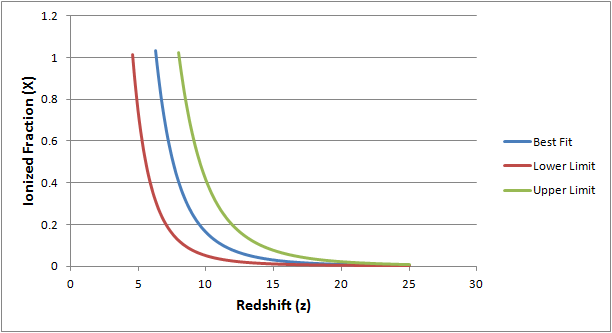
\includegraphics[width=\textwidth]{F:/Extragalactic cosmology/IonizedFraction1.png}
		\caption{Plot of modeled ionized fraction of the IGM as a function of redshift.} 
	\label{fig:IonizedFraction1}
\end{figure}

From this we get that the universe is completely ionized at a redshift $6.3\pm1.7$, ignoring the rather large errors, this number is not a bad estimate of the epoch. We know this from articles such as \cite{Ota:arXiv0707.1561} which show from observations of Lyman-$\alpha$ emitters that there must be a large ionized fraction at 6.5, due to attenuation from neutral hydrogen. Various theoretical models of star formation rate predict a ionized universe at around 6 and from \cite{2012MNRAS.423..862K} it is stated that the Sunyaev-Zeldovich effect has put a limit that Reionization ends earlier than 5.8.\\
However as recombination has not been included which will slow down the rate at which the universe is ionized or the fact that both the escape fraction and $\zeta$ are likely to change with redshift, this number is not actually realistic.\\

\subsection{Evolving Escape Fraction}
As already stated the previous results make a basic assumption of of the escape fraction to be about $20\%$ during the epoch of reionization. This is obviously not a very good assumption as it will evolve with redshift. However there lies a problem in this which is related to the previous section, 
%Beth's bit on fesc
which explained the difficulty in measuring this parameter as well as the problems in extrapolating out to higher redshifts much like in our star formation rates. This uncertainty in the measure is what leads to the differences stated in \cite{2012ApJ...759L..38A}, which states a higher fraction at higher redshift due to lack of dust, and \cite{2000ApJ...545...86W} which states the opposite, due to increasing disk densities and increasing density in the universe as a whole. However from \cite{2012arXiv1209.2123F} and \cite{2013MNRAS.428L...1M} by using recent semi-analytical model they found that the escape fraction does indeed increase with redshift and so this is the model that is used in this project.\\
Once again using the fit program to fit a exponential to the escape fraction measurements and predictions from \cite{2012ApJ...759L..38A}, \cite{2006ApJ...651L..89R} and \cite{2006MNRAS.371L...1I}. The functional form that is achieved is,
\begin{equation}   
f_{esc}(z)=e^{0.013\pm0.011-0.952\pm0.06}
\end{equation}
The code is then run again with this escape fraction instead of the constant $20\%$, the results achieved are shown in \ref{fig:IonizedFraction2}

\begin{figure}
	\centering
		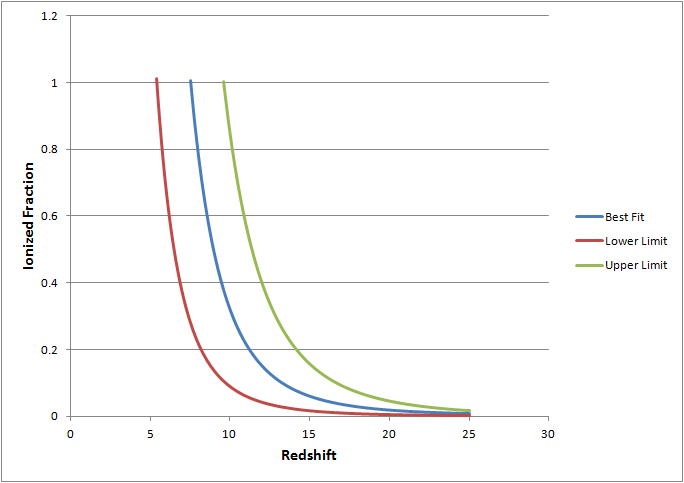
\includegraphics[width=\textwidth]{F:/Extragalactic cosmology/IonizedFraction2.png}
		\caption{Plot of modeled ionized fraction of the IGM as a function of redshift with predicting evolving escape fraction.} 
	\label{fig:IonizedFraction2}
\end{figure}

This graph shows that the addition of the evolving escape fraction has resulted in the universe being ionized quicker which is what is expected, since recombinations have not been included in this model. This model outputs a redshift of $7.5\pm2.1$, which shows the increase in redshift and also in error due to the error on $f_{esc}$ itself. It is very hard to determine whether this is an improvement or a hindrance to the previous model just due to the uncertainty on measuring/predicting $f_{esc}$, therefore it is hard to be certain of accuracy of the evolving form of $f_{esc}$.\\


@ARTICLE{2010Natur.468...49R,
   author = {{Robertson}, B.~E. and {Ellis}, R.~S. and {Dunlop}, J.~S. and 
	{McLure}, R.~J. and {Stark}, D.~P.},
    title = "{Early star-forming galaxies and the Reionization of the Universe}",
%  journal = {\nat},
archivePrefix = "arXiv",
   eprint = {1011.0727},
 primaryClass = "astro-ph.CO",
     year = 2010,
    month = nov,
   volume = 468,
    pages = {49-55},
      doi = {10.1038/nature09527},
   adsurl = {http://adsabs.harvard.edu/abs/2010Natur.468...49R},
  adsnote = {Provided by the SAO/NASA Astrophysics Data System}
}

@ARTICLE{2011ApJS..192...18K,
   author = {{Komatsu}, E. and {Smith}, K.~M. and {Dunkley}, J. and {Bennett}, C.~L. and 
	{Gold}, B. and {Hinshaw}, G. and {Jarosik}, N. and {Larson}, D. and 
	{Nolta}, M.~R. and {Page}, L. and {Spergel}, D.~N. and {Halpern}, M. and 
	{Hill}, R.~S. and {Kogut}, A. and {Limon}, M. and {Meyer}, S.~S. and 
	{Odegard}, N. and {Tucker}, G.~S. and {Weiland}, J.~L. and {Wollack}, E. and 
	{Wright}, E.~L.},
    title = "{Seven-year Wilkinson Microwave Anisotropy Probe (WMAP) Observations: Cosmological Interpretation}",
%  journal = {\apjs},
archivePrefix = "arXiv",
   eprint = {1001.4538},
 primaryClass = "astro-ph.CO",
 keywords = {cosmic background radiation, cosmology: observations, dark matter, early universe, space vehicles},
     year = 2011,
    month = feb,
   volume = 192,
      eid = {18},
    pages = {18},
      doi = {10.1088/0067-0049/192/2/18},
   adsurl = {http://adsabs.harvard.edu/abs/2011ApJS..192...18K},
  adsnote = {Provided by the SAO/NASA Astrophysics Data System}
}

@ARTICLE{2010MNRAS.401.2561W,
   author = {{Wyithe}, J.~S.~B. and {Hopkins}, A.~M. and {Kistler}, M.~D. and 
	{Y{\"u}ksel}, H. and {Beacom}, J.~F.},
    title = "{Determining the escape fraction of ionizing photons during Reionization with the GRB-derived star formation rate}",
 % journal = {\mnras},
archivePrefix = "arXiv",
   eprint = {0908.0193},
 primaryClass = "astro-ph.CO",
 keywords = {galaxies: high-redshift, intergalactic medium, diffuse radiation, cosmology: theory, large scale structure of Universe},
     year = 2010,
    month = feb,
   volume = 401,
    pages = {2561-2571},
      doi = {10.1111/j.1365-2966.2009.15834.x},
   adsurl = {http://adsabs.harvard.edu/abs/2010MNRAS.401.2561W},
  adsnote = {Provided by the SAO/NASA Astrophysics Data System}
}
	
@ARTICLE{2012ApJ...759L..38A,
   author = {{Alvarez}, M.~A. and {Finlator}, K. and {Trenti}, M.},
    title = "{Constraints on the Ionizing Efficiency of the First Galaxies}",
%  journal = {\apjl},
archivePrefix = "arXiv",
   eprint = {1209.1387},
 primaryClass = "astro-ph.CO",
 keywords = {cosmology: theory, dark ages, Reionization, first stars, intergalactic medium},
     year = 2012,
    month = nov,
   volume = 759,
      eid = {L38},
    pages = {L38},
      doi = {10.1088/2041-8205/759/2/L38},
   adsurl = {http://adsabs.harvard.edu/abs/2012ApJ...759L..38A},
  adsnote = {Provided by the SAO/NASA Astrophysics Data System}
}  

%@ARTICLE{2006A&A...459..745F,
   author = {{Fontana}, A. and {Salimbeni}, S. and {Grazian}, A. and {Giallongo}, E. and 
	{Pentericci}, L. and {Nonino}, M. and {Fontanot}, F. and {Menci}, N. and 
	{Monaco}, P. and {Cristiani}, S. and {Vanzella}, E. and {de Santis}, C. and 
	{Gallozzi}, S.},
    title = "{The Galaxy mass function up to z =4 in the GOODS-MUSIC sample: into the epoch of formation of massive galaxies}",
%  journal = {\aap},
   eprint = {arXiv:astro-ph/0609068},
 keywords = {galaxies: distances and redshift, galaxies: evolution, galaxies: high-redshift, galaxies: fundamental parameters, galaxies: luminosity fuction, mass function},
     year = 2006,
    month = dec,
   volume = 459,
    pages = {745-757},
      doi = {10.1051/0004-6361:20065475},
   adsurl = {http://adsabs.harvard.edu/abs/2006A%26A...459..745F},
  adsnote = {Provided by the SAO/NASA Astrophysics Data System}
}

%@ARTICLE{2003A&A...401...73W,
   author = {{Wolf}, C. and {Meisenheimer}, K. and {Rix}, H.-W. and {Borch}, A. and 
	{Dye}, S. and {Kleinheinrich}, M.},
%    title = "{The COMBO-17 survey: Evolution of the galaxy luminosity function from 25 000 galaxies with 0.2{\lt} z {\lt}1.2}",
%  journal = {\aap},
   eprint = {arXiv:astro-ph/0208345},
 keywords = {techniques: photometric, surveys, galaxies: evolution, galaxies: distances and redshifts},
     year = 2003,
    month = apr,
   volume = 401,
    pages = {73-98},
      doi = {10.1051/0004-6361:20021513},
   adsurl = {http://adsabs.harvard.edu/abs/2003A%26A...401...73W},
  adsnote = {Provided by the SAO/NASA Astrophysics Data System}
}

@ARTICLE{2003ApJS..149..289B,
   author = {{Bell}, E.~F. and {McIntosh}, D.~H. and {Katz}, N. and {Weinberg}, M.~D.
	},
    title = "{The Optical and Near-Infrared Properties of Galaxies. I. Luminosity and Stellar Mass Functions}",
 % journal = {\apjs},
   eprint = {arXiv:astro-ph/0302543},
 keywords = {Galaxies: Evolution, Galaxies: General, Galaxies: Luminosity Function, Mass Function, Galaxies: Stellar Content},
     year = 2003,
    month = dec,
   volume = 149,
    pages = {289-312},
      doi = {10.1086/378847},
   adsurl = {http://adsabs.harvard.edu/abs/2003ApJS..149..289B},
  adsnote = {Provided by the SAO/NASA Astrophysics Data System}
}

@article {Ota:arXiv0707.1561,
author="Kazuaki Ota and Masanori Iye and Nobunari Kashikawa and Kazuhiro Shimasaku and Masakazu A. R. Kobayashi and Tomonori Totani and Masahiro Nagashima and Tomoki Morokuma and Hisanori Furusawa and Takashi Hattori and Yuichi Matsuda and Tetsuya Hashimoto and Masami Ouchi",
title="The Reionization and Galaxy Evolution Probed by z=7 Lyman Alpha Emitters",
year="2007",
eprint="arXiv/0707.1561",
doi="10.1393/ncb/i2008-10435-8"
} 

@ARTICLE{2012MNRAS.423..862K,
   author = {{Kuhlen}, M. and {Faucher-Gigu{\`e}re}, C.-A.},
    title = "{Concordance models of reionization: implications for faint galaxies and escape fraction evolution}",
%  journal = {\mnras},
archivePrefix = "arXiv",
   eprint = {1201.0757},
 primaryClass = "astro-ph.CO",
 keywords = {galaxies: dwarf, galaxies: formation, galaxies: high-redshift, intergalactic medium, cosmology: theory, dark ages, reionization, first stars},
     year = 2012,
    month = jun,
   volume = 423,
    pages = {862-876},
      doi = {10.1111/j.1365-2966.2012.20924.x},
   adsurl = {http://adsabs.harvard.edu/abs/2012MNRAS.423..862K},
  adsnote = {Provided by the SAO/NASA Astrophysics Data System}
}

@ARTICLE{2000ApJ...545...86W,
   author = {{Wood}, K. and {Loeb}, A.},
    title = "{Escape of Ionizing Radiation from High-Redshift Galaxies}",
%  journal = {\apj},
   eprint = {arXiv:astro-ph/9911316},
 keywords = {Galaxies: Formation, ISM: H II Regions, Galaxies: Quasars: General},
     year = 2000,
    month = dec,
   volume = 545,
    pages = {86-99},
      doi = {10.1086/317775},
   adsurl = {http://adsabs.harvard.edu/abs/2000ApJ...545...86W},
  adsnote = {Provided by the SAO/NASA Astrophysics Data System}
}

@ARTICLE{2012arXiv1209.2123F,
   author = {{Ferrara}, A. and {Loeb}, A.},
    title = "{Escape Fraction of Ionizing Radiation from Starburst Galaxies at High Redshifts}",
  journal = {ArXiv e-prints},
archivePrefix = "arXiv",
   eprint = {1209.2123},
 primaryClass = "astro-ph.CO",
 keywords = {Astrophysics - Cosmology and Extragalactic Astrophysics},
     year = 2012,
    month = sep,
   adsurl = {http://adsabs.harvard.edu/abs/2012arXiv1209.2123F},
  adsnote = {Provided by the SAO/NASA Astrophysics Data System}
}

@ARTICLE{2013MNRAS.428L...1M,
   author = {{Mitra}, S. and {Ferrara}, A. and {Choudhury}, T.~R.},
    title = "{The escape fraction of ionizing photons from high-redshift galaxies from data-constrained reionization models}",
%  journal = {\mnras},
archivePrefix = "arXiv",
   eprint = {1207.3803},
 primaryClass = "astro-ph.CO",
 keywords = {intergalactic medium, cosmology: theory, dark ages, reionization, first stars, large-scale structure of Universe},
     year = 2013,
    month = jan,
   volume = 428,
    pages = {L1-L5},
      doi = {10.1093/mnrasl/sls001},
   adsurl = {http://adsabs.harvard.edu/abs/2013MNRAS.428L...1M},
  adsnote = {Provided by the SAO/NASA Astrophysics Data System}
}

@ARTICLE{2006ApJ...651L..89R,
   author = {{Razoumov}, A.~O. and {Sommer-Larsen}, J.},
    title = "{Escape of Ionizing Radiation from Star-forming Regions in Young Galaxies}",
%  journal = {\apjl},
   eprint = {arXiv:astro-ph/0609545},
 keywords = {Galaxies: Formation, Galaxies: Intergalactic Medium, ISM: H II Regions, Radiative Transfer},
     year = 2006,
    month = nov,
   volume = 651,
    pages = {L89-L92},
      doi = {10.1086/509636},
   adsurl = {http://adsabs.harvard.edu/abs/2006ApJ...651L..89R},
  adsnote = {Provided by the SAO/NASA Astrophysics Data System}
}

@ARTICLE{2006MNRAS.371L...1I,
   author = {{Inoue}, A.~K. and {Iwata}, I. and {Deharveng}, J.-M.},
    title = "{The escape fraction of ionizing photons from galaxies at z = 0-6}",
%  journal = {\mnras},
   eprint = {arXiv:astro-ph/0605526},
 keywords = {galaxies: evolution: intergalactic medium: cosmology: observations: diffuse radiation, galaxies: evolution, intergalactic medium, cosmology: observations, diffuse radiation},
     year = 2006,
    month = sep,
   volume = 371,
    pages = {L1-L5},
      doi = {10.1111/j.1745-3933.2006.00195.x},
   adsurl = {http://adsabs.harvard.edu/abs/2006MNRAS.371L...1I},
  adsnote = {Provided by the SAO/NASA Astrophysics Data System}
}

@ARTICLE{2012ApJ...746..125H,
   author = {{Haardt}, F. and {Madau}, P.},
    title = "{Radiative Transfer in a Clumpy Universe. IV. New Synthesis Models of the Cosmic UV/X-Ray Background}",
  journal = {\apj},
archivePrefix = "arXiv",
   eprint = {1105.2039},
 primaryClass = "astro-ph.CO",
 keywords = {cosmology: theory, diffuse radiation, intergalactic medium, galaxies: evolution, quasars: general},
     year = 2012,
    month = feb,
   volume = 746,
      eid = {125},
    pages = {125},
      doi = {10.1088/0004-637X/746/2/125},
   adsurl = {http://adsabs.harvard.edu/abs/2012ApJ...746..125H},
  adsnote = {Provided by the SAO/NASA Astrophysics Data System}
}

@ARTICLE{2011MNRAS.412L..16R,
   author = {{Rai{\v c}evi{\'c}}, M. and {Theuns}, T.},
    title = "{Modelling recombinations during cosmological reionization}",
%  journal = {\mnras},
 keywords = {radiative transfer, methods: numerical, cosmology: dark ages, reionization, first stars},
     year = 2011,
    month = mar,
   volume = 412,
    pages = {L16-L19},
      doi = {10.1111/j.1745-3933.2010.00993.x},
   adsurl = {http://adsabs.harvard.edu/abs/2011MNRAS.412L..16R},
  adsnote = {Provided by the SAO/NASA Astrophysics Data System}
}

@ARTICLE{2006MNRAS.373.1265O,
   author = {{Oppenheimer}, B.~D. and {Dav{\'e}}, R.},
    title = "{Cosmological simulations of intergalactic medium enrichment from galactic outflows}",
%  journal = {\mnras},
   eprint = {arXiv:astro-ph/0605651},
 keywords = {methods: numerical, galaxies: formation, galaxies: high-redshift, intergalactic medium, cosmology: theory},
     year = 2006,
    month = dec,
   volume = 373,
    pages = {1265-1292},
      doi = {10.1111/j.1365-2966.2006.10989.x},
   adsurl = {http://adsabs.harvard.edu/abs/2006MNRAS.373.1265O},
  adsnote = {Provided by the SAO/NASA Astrophysics Data System}
}


\end{document}     